% https://drive.google.com/file/d/0B3FgdUXk8fTrNWUwQ0tpLWFsbE0/view?usp=sharing

\begin{figure}[H]
  \centering
  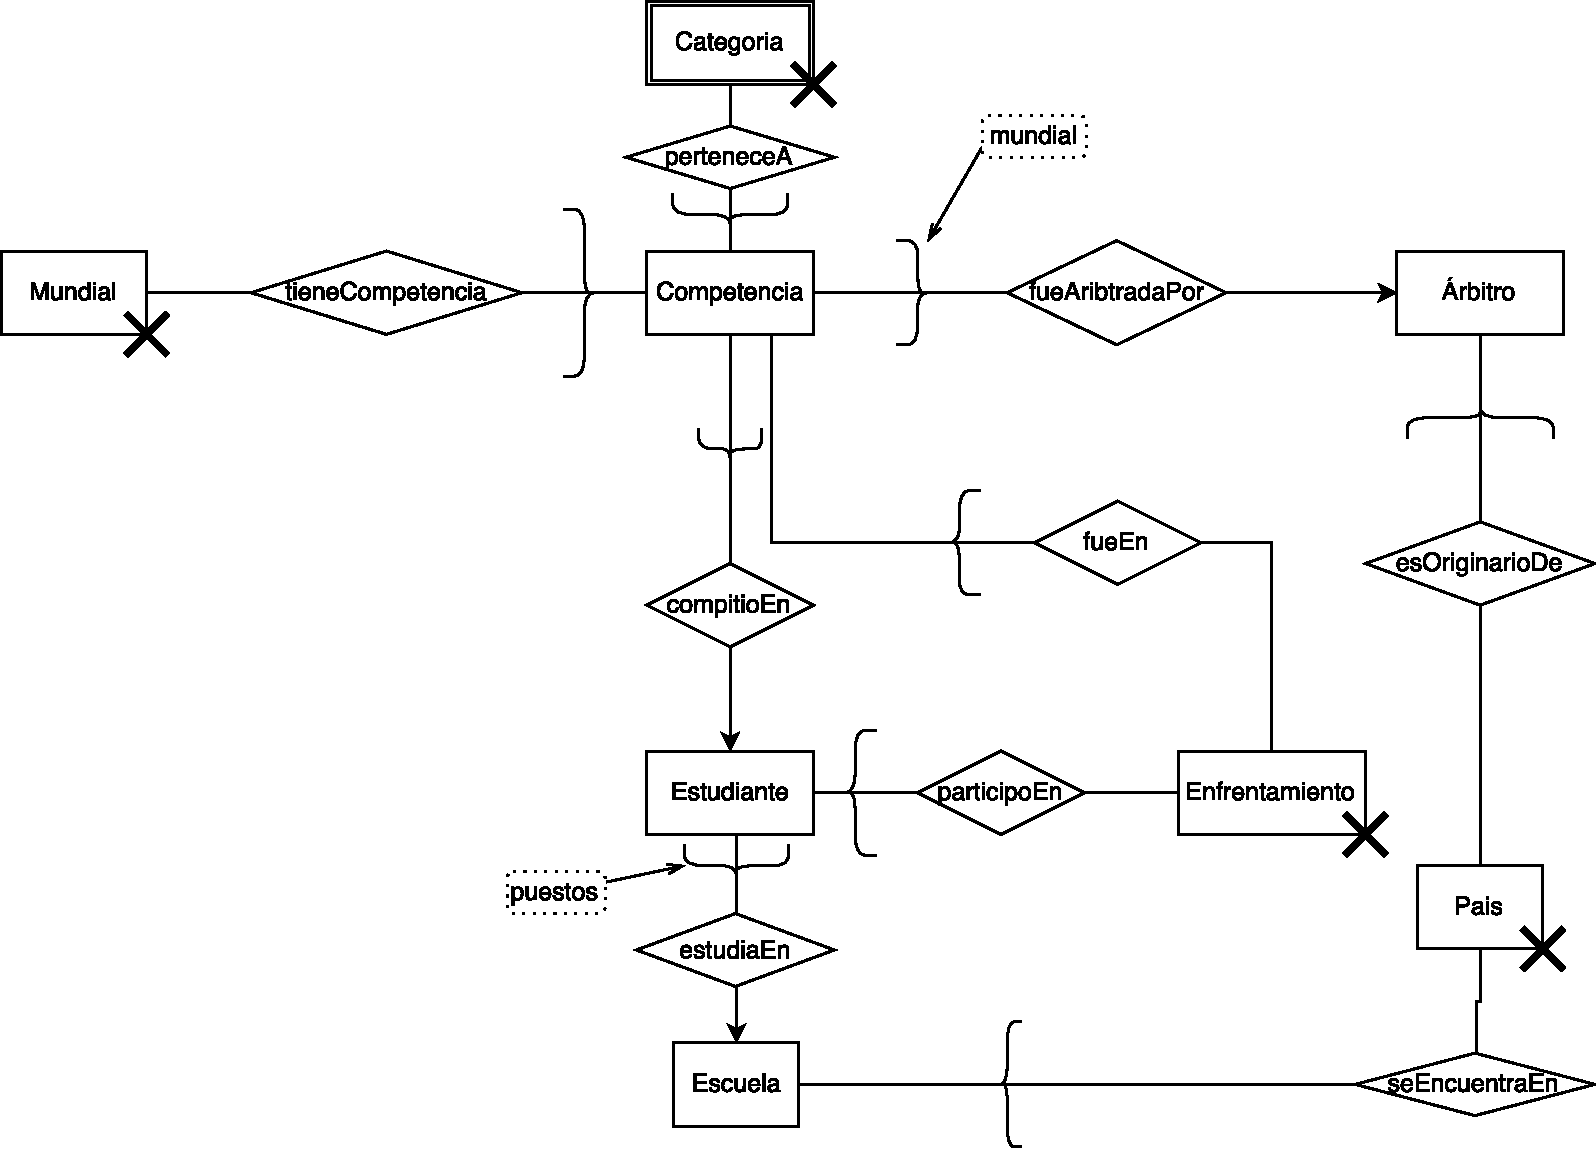
\includegraphics[width=\textwidth]{img/did.pdf}
  \caption{Diagrama de Interacción de Documentos. Se omiten atributos y cardinalidad de las relaciones por simplicidad, pero son las mismas que en el diagrama de entidad relación.}
\end{figure}

Notemos que las entidades que tendremos en nuestro json schema (y por lo tanto en nuestra base de datos) serán solamente cuatro: Competencia, Árbitro, Estudiante y Escuela.

Cuando embebemos entidades en otras lo hacemos sobre todo para poder cumplir con las queries y además hacerlo de manera eficiente.

Por ejemplo, embebemos los puestos de los estudiantes en escuela para poder hacer rápidamente la query 2.2 (\textit{La cantidad de medallas por nombre de escuela en toda la historia}).

Similarmente, embebemos el mundial de la competencia en Árbitro para poder realizar la query 2.4 (\textit{Los árbitros que participaron en al menos 4 campeonatos}) de manera eficiente.

La eliminación de las entidades País y Categoría es muy razonable. Eliminamos también Mundial porque no es particularmente necesaria para ninguna query y no vale la pena duplicar la información. Finalmente, eliminamos Enfrentamiento, porque es redundante tenerla (dado que embeberla en Estudiante y en Competencia nos da toda la información que eventualmente podramos necesitar).
